\section{Metode}
	\begin{figure}[h!]
	\centering
	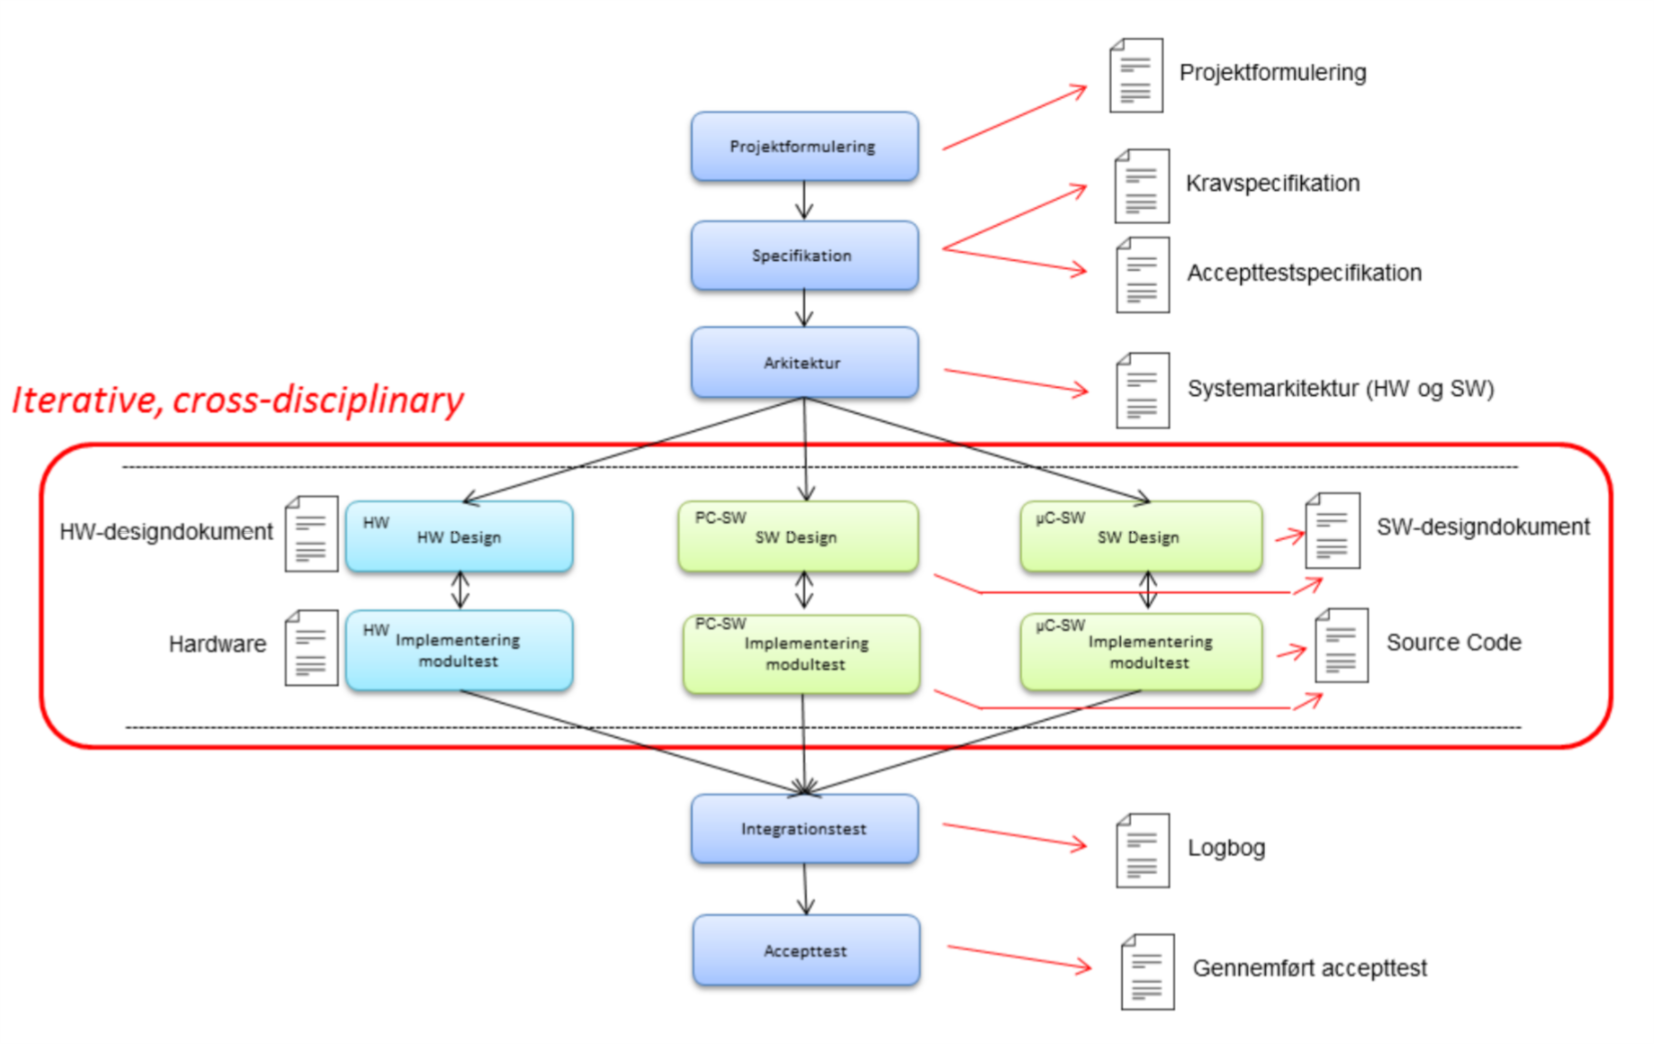
\includegraphics[width=0.8\linewidth]{Udviklingsproces/ASEmodellen}
	\caption{ASE-modellen \cite{ASE}}
	\label{fig:ase-modellen}
\end{figure}

I dette semesterprojekt har vi arbejdet ud fra ASE-udviklingsmodellen, der kan ses på figur \vref{fig:ase-modellen}. Denne model er en kombination af vandfaldsmodellen og v-modellen. V-modellen kommer til udtryk ved specifikationen, hvor vi udformer krav i kravspecifikationen samtidig med, at vi udformer tests i accepttestspecifikationen. Ved at gøre dette sideløbende sikrer vi, at de krav, der bliver stillet er testbare. Vandfaldsmodellen kommer til udtryk i design og implementeringsfasen. I denne fase forløber projektet i iterationer. Dette gør vi for kontinuerligt at kunne justere og optimere produktet ud fra tidligere iterationer. 
 
Vi har igennem udviklingsprojektet benyttet os af review på kravspecifikationen, accepttest, hardware arkitektur og software arkitektur. Reviewet er foregået med de resterende grupper på semesterprojektet. Begge grupper læste og kommenterede på det emne der skulle reviewes. Derefter mødtes grupperne til et møde, hvor eventuelle kommentarer blev forklaret og diskuteret. Grundet at reviewgrupperne på forhånd ved, hvad systemet omhandler, har vi derfor ikke kunne få et optimalt billede af, hvorvidt vores dokumentation er forståelig for en potentiel kunde. Dog har reviewene givet os et billede af, hvordan man kan udforme projektet på flere måder. Vi har fået feedback, der har hjulpet os til at spore os ind på den opsætning vi synes er den rette for vores system.   

\subsection{Samarbejdsaftale}
Vi har anvendt en samarbejdsaftale, som er udarbejdet i fællesskab i gruppen. Formålet med at udarbejde en samarbejdsaftale er dels at få lavet en forventningsafstemning omkring ambitionsniveauet og arbejdsindsatsen for hvert gruppemedlem for projektet. Disse krav er formuleret således:
\begin{itemize}
	\item 6.1 Alle medlemmer i gruppen har et ambitionsniveau på omkring middel på karakterskalaen. 
	\item 6.2 Gruppen arbejder min. 3 timer om ugen i fællesskab og derudover er der forberedelse og hjemmearbejde. 
\end{itemize}

 Hvis de opstillede krav ikke blev opfyldt af et gruppemedlem, ville samarbejdskontrakten have været udfordret, og derfor ville der have været brug for et punkt i samarbejdskontrakten omkring konflikthåndtering. Derfor har vi valgt at formulere en procedure i forhold til hvad der skal ske, hvis der opstår en konflikt. Disse procedure er formuleret således: 
 \begin{itemize}
 	\item 5.1 Ved 3 udeblivelser uden gyldig begrundelse fra gruppemøder, hvis arbejdsmoralen er lav, eller arbejdsindsatsen ikke er tilstrækkelig ift. gruppens ambitionsniveau, tager Thea en snak med gruppemedlemmet. Her forklares hvad konflikten går ud på, og hvordan gruppemedlemmet kan løse konflikten sammen med gruppen.
 		\item  5.1.1 Hvis konfrontationen ikke ændrer på gruppemedlemmets aktivitet i projektet, løses konflikten med hjælp fra vejlederen. 
\end{itemize}
 
  Dog har vi ikke haft nogle konflikter i gruppen, og dermed har vores samarbejdskontrakt ikke været udfordret. 

Derudover indeholder samarbejdskontrakten punkter omkring hvornår der afholdes gruppemøde og vejledermøde samt proceduren for afbud til disse. Dette kan ses i samarbejdskontrakten. 


\subsection{Udviklingsforløb}\label{sec:udvikling}
Som arbejdsmetoden i dette projekt har vi anvendt Scrum. Vi har valgt at fokusere på de dele af scrum, der har været relevant i forhold til vores projekt. Vi har valgt at have en product backlog og en sprint backlog. Derudover har vi haft rollerne scrum-master og scrum-team. Vores projektleder Sarah Krohn Fenger har fungeret som scrum-master. Denne rolle har indeholdt opgaverne som ansvarlig for planlægning af sprint, review af sprint og ordstyring af de to ugentlige standup-møder. Hvert sprint har varet en uge. Derfor har vi én gang ugentligt holdt et gruppemøde. Gruppemødet blev sædvanligvis holdt onsdag morgen og til dette møde har vi lavet review af det forrige sprint og planlagt det næste sprint for den kommende uge. Ved review af sprintet har der været fokus på, hvad der er færdiggjort samt scrum-teamets oplevelse af, hvad der er gået godt og hvordan eventuelle problemer er løst. Ved planlægning af sprintet har fokus været, hvad der skal laves og hvad målet for den kommende uge er. Både review af sprintet og planlægning af næste sprint dokumenteres således, at det er tilgængeligt for scrum-teamet. Dokumentationen kan ses i bilag x.

	\begin{figure}[h!]
	\centering
	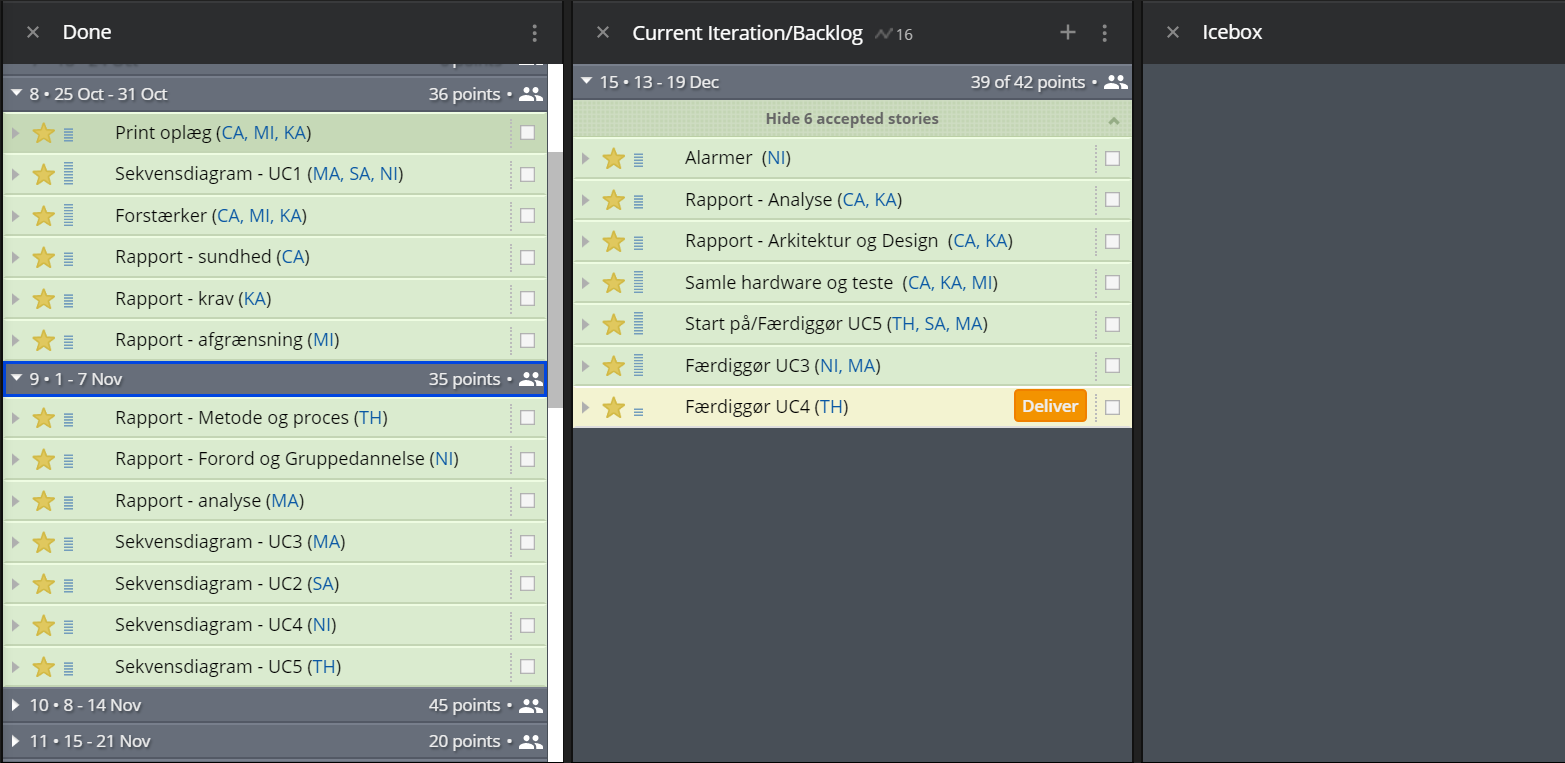
\includegraphics[width=0.9\linewidth]{Udviklingsproces/Metode/PivotalTracker}
	\label{fig:pivotal}
	\caption{Screenshot af Pivotal Tracker}
\end{figure}

På figur \vref{fig:pivotal} ses et screenshot af programmet Pivotal Tracker. Pivotal Tracker er et program, hvor et projekt kan inddeles i mindre opgaver. Disse opgaver placeres i "icebox". Når sprintet planlægges, kigges der på de opgaver der allerede befinder sig i "icebox". Det vurderes, hvilke opgaver der skal startes på og hvorvidt der skal tilføjes flere opgaver til "icebox". Opgaverne tildeles point alt efter, hvor lang tid det vurderes, at der skal bruges på opgaven. De opgaver der startes placerer sig automatisk i "current backlog". Ved review af sprint kigges der på, hvilke opgaver i "current backlog", der er færdige. Disse opgaver markeres herefter færdige, og flyttes dermed til "done". 

Udover gruppemøder har vi to gange om ugen haft standup-møder. Formålet med standup-møder har været at få en status på, hvor langt teamet har været med de forskellige opgaver samt, om der har været problemer, og hvordan disse har kunne løses. Derudover har standup-møderne været med til at give Sarah et billede af om tidsplanen skulle opdateres. Til at konfigurere tidsplanen har vi brugt Team Gantt. Tidsplanen kan ses i bilag xx. Et eksempel på dette ses nedenfor. 

	\begin{figure}[h!]
	\centering
	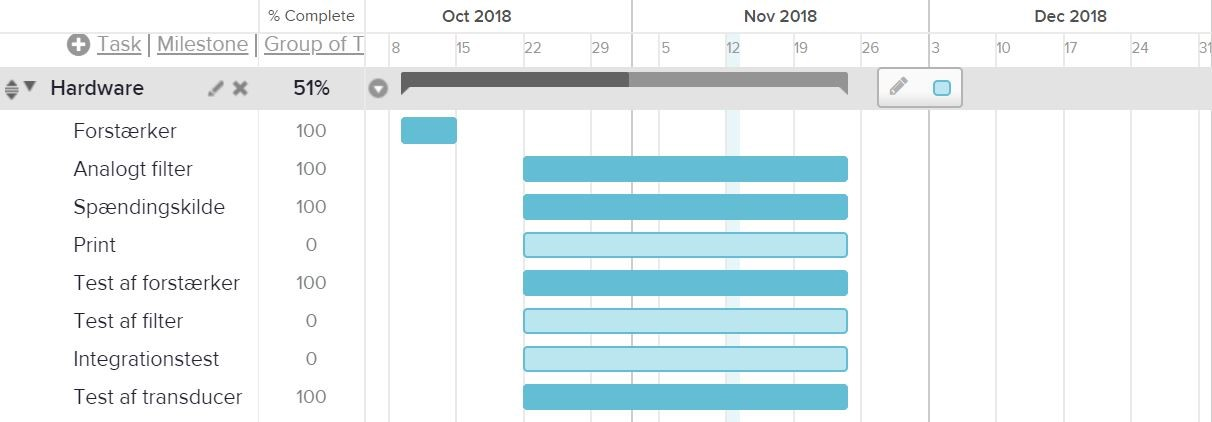
\includegraphics[width=0.9\linewidth]{Udviklingsproces/Metode/TeamGantt}
	\label{fig:teamgantt}
	\caption{Screenshot af TeamGantt}
\end{figure}

Sarah har stået for at opdatere tidsplanen, og har dermed kunne forholde sig til, hvornår teamet skulle bruge flere timer i projektet, så opgaverne blev fuldført. Udover opdatering af tidsplan og tovholder på sprint review samt sprint planlægning har Sarahs opgaver været mødeindkaldelse til gruppemøder samt referent til disse. I forhold til lederrollen har gruppen ikke givet Sarah beføjelser. Sarahs opgaver som leder har primært været at være tovholder på projektet. 

\subsection{Arbejdsfordeling}
Gruppen tog en beslutning om at fordele projektarbejdet i to teams; et softwareteam og et hardwareteam, da projektet er så stort at det ikke er muligt at være inde over det hele. Softwareteamet er bestående af Mathias, Nicolai og Thea, mens Hardwareteamet er bestående af Caroline, Kajene og Mikkel. Sarahs rolle er flyver, som skiftevis er med softwareteamet og hardwareteamet, alt afhængigt af hvor der er brug for ekstra hjælp. Vi fandt dog hurtigt ud af, at Software-gruppen havde mest brug for hjælp og derfor har Sarah været en del af denne siden uge 3 af projektet dvs. Sarah nåede at hjælpe hardware 1 uge.

Denne opdeling har fungeret udmærket, da den har givet mulighed for at specialisere sig, og komme dybere ned i stoffet. Dog har det også givet anledning til frustration i forhold til ikke at være helt inde over hvad det modsatte team arbejder med. De ugentlige standup-møder har bidraget til at begge teams får en forståelse for hvad der bliver arbejdet med i både hardware og software.

Projektarbejdet er også blevet uddelegeret, så hvert gruppemedlem har fået primære og sekundære områder, arbejdsfordelingen i detaljer ses i et skema i bilaget "arbejdsfordeling".

















